\begin{frame}
    \frametitle{MRCPP features}
    \begin{itemize}
        \item Currently: precision based
        \item All grids are function specific
        \item On the fly adaptivity
        \item Complicated algorithms
        \item Difficult to load balance
    \end{itemize}
    \vspace{5mm}
    \begin{itemize}
        \item Future: grid based
        \item Fixed grids in each SCF iteration
        \item Grid refinement between iterations
        \item Fixed grids $\longrightarrow$ better performance
        \item Better error control for \emph{local} operators
    \end{itemize}
\end{frame}

\begin{frame}
    \frametitle{Local operators}
    \begin{columns}
    \begin{column}{0.3\linewidth}
    \normalsize
    \centering
    \begin{equation}
        \nonumber
        \rho \longrightarrow \nabla \rho
    \end{equation}
    
    \vspace{3mm}

    \begin{equation}
        \nonumber
        \rho \longrightarrow E_{xc}
    \end{equation}
    
    \vspace{2mm}

    \begin{equation}
        \nonumber
        \rho \longrightarrow \frac{\delta E_{xc}}{\delta \rho}
    \end{equation}
    
    \vspace{1mm}

    \begin{equation}
        \nonumber
        \rho \longrightarrow \frac{\delta^2 E_{xc}}{\delta \rho^2}
    \end{equation}
    
    \vspace{5mm}

    \end{column}
    \begin{column}{0.7\linewidth}
    \centering

    Treutler and Ahlrichs claim that the error $\Delta E_{xc}$ in the XC 
    energy\\ is related to the error $\Delta N$ in the charge integral

    \vspace{3mm}

    \begin{equation}
        \nonumber
        |\Delta E_{xc}| \leq\Delta N
    \end{equation}

    \vspace{5mm}

    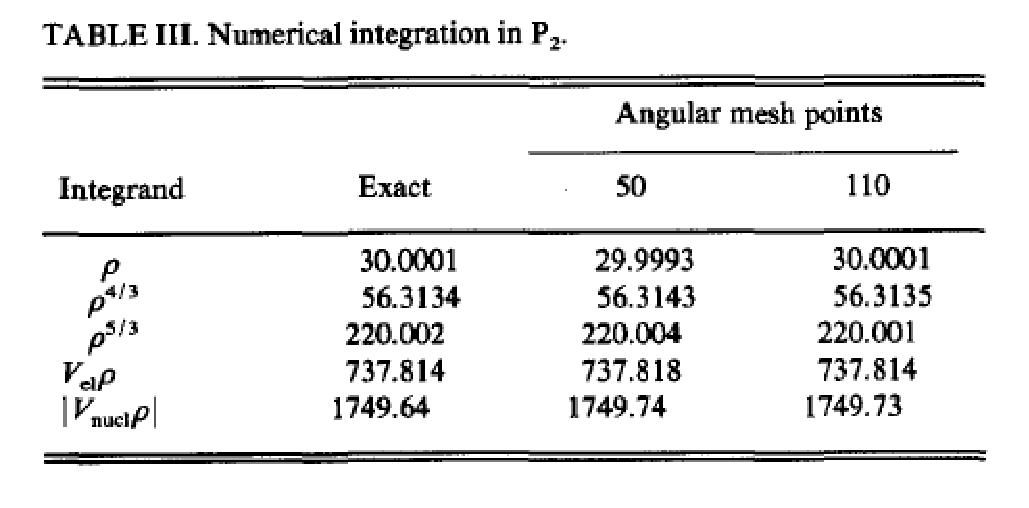
\includegraphics[scale = 0.4]{figures/beckeAccuracy.pdf}

    \vspace{1mm}

    \scriptsize
    A. D. Becke, 
    {\it JCP}, \textbf{88} (4), 1988

    \end{column}
    \end{columns}
\end{frame}

\begin{frame}
    \frametitle{MRGrid features}
    \hspace{45mm} \textbf{Basic}
    \begin{columns}
    \begin{column}{0.3\linewidth}
    \end{column}
    \begin{column}{0.5\linewidth}
    \begin{itemize}
        \item generateGrid(molecule)
        \item getQuadraturePoints()
        \item getQuadratureValues()
        \item getQuadratureWeights()
    \end{itemize}
    \end{column}
    \begin{column}{0.2\linewidth}
    \end{column}
    \end{columns}

    \vspace{15mm}

    \begin{columns}
    \begin{column}{0.1\linewidth}
    \end{column}
    \begin{column}{0.4\linewidth}
    \hspace{5mm} \textbf{More advanced}
    \begin{itemize}
        \item project(function)
        \item estimateError()
        \item refineGrid(prec)
        \item integrate()
        \item innerProduct()
        \item arithmetic operations
        \item Coulomb operator
    \end{itemize}
    \end{column}
    \begin{column}{0.5\linewidth}
    \hspace{5mm} \textbf{Algorithm}
    \begin{itemize}
        \item Generate initial grid
        \item \textbf{Start SCF cycle}
        \item Project density
        \item Compute potentials
        \item Estimate errors
        \item \textbf{Finish SCF cycle}
        \item Refine grids if necessary
    \end{itemize}
    \end{column}
    \end{columns}
\end{frame}

